% \documentclass[10pt]{beamer}
\documentclass[10pt,usenames,dvipsnames]{beamer}

\usepackage{graphicx}
\usepackage{amsmath}
\usepackage{amssymb}
\usepackage{algorithm,algorithmic}
\usepackage{float}
\usepackage{caption}
\usepackage{cleveref}
\usepackage[normalem]{ulem}

\usepackage[natbib=true,backend=bibtex]{biblatex}
\addbibresource{ressources.bib}

\renewcommand\vec[1]{\boldsymbol{\mathbf {#1}}}
\newcommand\R{\mathbb {R}}
\newcommand\doubleminipage[2]{
\begin{figure}[H]
\centering
\centerline{
\begin{minipage}{0.5\textwidth}
    \caption*{\footnotesize GTN trained with \texttt{'base\_larger'}}%
    \includegraphics[trim=10 0 0 30,clip,width=\textwidth]{figures/base_larger_#1.pdf}
\end{minipage}%
\begin{minipage}{0.5\textwidth}
    \caption*{\footnotesize GTN trained with \texttt{'base\_larger3'}}%
    \includegraphics[trim=0 0 10 30,clip,width=\textwidth]{figures/base_larger3_#1.pdf}
\end{minipage}
}
\caption{#2%
\label{fig:results_#1}
}
\end{figure}
}


\usetheme[progressbar=frametitle]{metropolis}
\setbeamertemplate{section in toc}[sections numbered]
\usepackage{appendixnumberbeamer}


\usepackage{booktabs}
\usepackage[scale=2]{ccicons}

\usepackage{pgfplots}
\usepgfplotslibrary{dateplot}

\usepackage{xspace}
\newcommand{\themename}{\textbf{\textsc{metropolis}}\xspace}

\title{
Evaluating the Robustness of \\
Generative Teaching Networks
% Generative Teaching Networks: \\
% Accelerating Neural Architecture Search by Learning to Generate Synthetic Training Data
}
\subtitle{Felipe Petroski Such, Aditya Rawal, Joel Lehman, Kenneth O. Stanley, Jeff Clune}
\date{\today}
\author{Kurt Willis}
\institute{TU Berlin}
% \titlegraphic{\hfill\includegraphics[height=1.5cm]{logo.pdf}}

\begin{document}

\maketitle

\begin{frame}{Overview}
\large
\tableofcontents
\end{frame}


\section{Generative Teaching Networks}

\begin{frame}{Meta-Learning}
    \textbf{Meta-Learning} is about "learning to learn". 
    
    There are generally 3 components to Machine-Learning.. \\
    The \textbf{environment}, the learner \textbf{model} and the learning \textbf{algorithm}.
    
    % \nocite{*}
    % \printbibliography[keyword=meta,heading=none,]
\end{frame}

\begin{frame}{Generative Teaching Networks}
    \textit{Generative Teaching Networks} (GTN) aim to
    learn an environment and algorithm parameters
    via meta-learning
    for rapid training of a variety
    of different kinds of deep neural network architectures.
    \begin{center}
    \vspace*{10pt}
    \centerline{
    \only<2->{
    \begin{minipage}{0.5\textwidth}%
    \begin{tabular}{ l }%
        \textbf{traditional ML} \\
        \midrule
        environment: \texttt{fixed} \\  
        algorithm: \texttt{fixed} \\  
        model architecture: \texttt{fixed} \\
        model parameters: \texttt{learned}    
    \end{tabular}%
    \end{minipage}%
    }
    \only<-2>{
    \phantom{%
    \begin{minipage}{0.45\textwidth}%
    % \hspace*{20pt}
    \begin{tabular}{ l }%
        \textbf{Generative Teaching Networks} \\
        \midrule
        environment: \texttt{learned} \\  
        algorithm: \texttt{learned} \\  
        model architecture: \texttt{random} \\
        model parameters: \texttt{learned}    
    \end{tabular}%
    \end{minipage}%
    }
    }
    \only<3->{
    \begin{minipage}{0.45\textwidth}%
    % \hspace*{20pt}
    \begin{tabular}{ l }%
        \textbf{Generative Teaching Networks} \\
        \midrule
        environment: \texttt{learned} \\  
        algorithm: \texttt{learned} \\  
        model architecture: \texttt{random} \\
        model parameters: \texttt{learned}    
    \end{tabular}%
    \end{minipage}%
    }
    }
    \end{center}
\end{frame}

\begin{frame}{GTN Algorithm}
    \begin{algorithm}[H]
    \caption*{\textbf{Algorithm} Generative Teaching Networks}
    \begin{algorithmic}
    \STATE initialize $G_{\vec\omega}$
    \FOR{\texttt{2000 times}}
    \STATE sample $D_{\vec\theta}$
    \FOR{\texttt{64 times}}
        \STATE $\vec z = (\vec z_x, \vec z_y) \sim \text{sample randomly}$
        \STATE $\vec x \gets G_{\vec\omega}(\vec z)$
        \STATE $\hat {\vec y} \gets D_{\vec\theta}(\vec x)$
        \STATE ${\vec\theta} \gets {\vec\theta} - \lambda \nabla_{\vec\theta} \mathcal L(\hat{\vec y}, \vec z_y)$
    \ENDFOR
    \STATE ${\vec\omega} \gets {\vec\omega} - \gamma \nabla_{\vec\omega} \mathcal L(D_{\vec\theta}(\vec x_{\texttt{train}}), \vec y_{\texttt{train}})$
    \ENDFOR
    \end{algorithmic}
    \end{algorithm}
\end{frame}


\begin{frame}{Meta-Loop}
    \begin{figure}
        \centering
        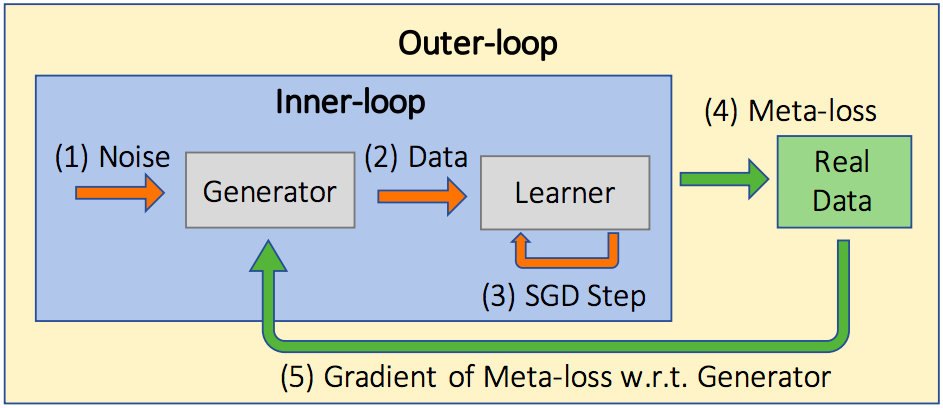
\includegraphics[width=\textwidth]{figures/Meta-Learning.png}
        \caption{Generative Teaching Networks meta-loop \cite{such2019generative}}
        % \label{fig:my_label}
    \end{figure}
\end{frame}

\begin{frame}{Full Curriculum}
    \textbf{Full Curriculum:} \\
    In addition to the weights of the generator $G$, the full ordered set of 64 latent vectors $\vec z^{(i)} \in \R^{138}$ and
    learning rates $\lambda^{(i)}$ (and weight decay parameters)
    are learned for $i \in [1,\ldots, 64]$.
\end{frame}

\begin{frame}{GTN - Results}
    \begin{figure}
        \centering
        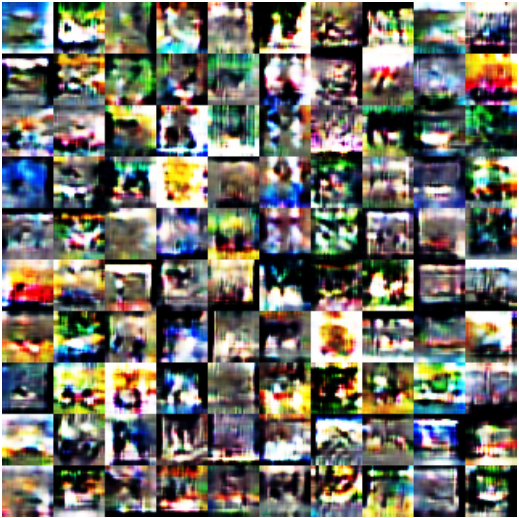
\includegraphics[width=0.5\textwidth]{figures/Examples.png}
        \caption{CIFAR10 Generator examples \cite{such2019generative}}
        % \label{fig:my_label}
    \end{figure}
\end{frame}

\begin{frame}{Experience With Codebase}
    \textit{Hope}: simply train a GTN, then use that to train custom models, however \ldots
    \begin{itemize}
        \item<2-> limited architecture choices (weight normalization necessary)
        \item<3-> pooling layer doesn't seem to work
        \item<4-> CIFAR10 performance too low
        \item<5-> attempt to recreate inner training loop failed
        \item<6-> custom autograd (required for gradient checkpointing) 
        \item<7-> custom convolution operation, only works on GPU
        \item<8-> extremely convoluted, interdependent code (functions inside of functions inside of functions)
    \end{itemize}
    \only<9->{$\rightarrow$ debugging \& interacting with code was very difficult.}
\end{frame}
\begin{frame}{Training Models}
    GTN trained on \texttt{'base\_larger'}.
    
    \only<-1>{\phantom{
    Criteria: mean accuracy over 5 independently trained networks should be $\geq 0.7$.}}
    \only<2->{
    \textit{Criteria}: mean accuracy over 5 independently trained networks should be $\geq 0.7$.}
    
    \begin{tabular}{l l l l}
    \only<2->{\textit{\hfill{learning algorithm }}&\texttt{10\_gtn} &\texttt{vanilla} &\texttt{gtn} }\\
    \textit{learner type} &&&\\
    \midrule
    \only<-4>{\texttt{'base'} \only<2->{&0.16 &0.95 &0.22 }\\}%
    \only<5->{\sout{\texttt{'base'}} \only<2->{&0.16 &0.95 &0.22 }\\}%
    \only<-3>{\texttt{'base\_fc'} \only<2->{&0.97 &0.98 &0.98 }\\}%
    \only<4->{\sout{\texttt{'base\_fc'}} \only<2->{&0.97 &0.98 &0.98 }\\}%
    \texttt{'base\_larger'} \only<2->{&0.97 &0.98 &0.98 }\\%
    \only<-4>{\texttt{'base\_larger2'} \only<2->{&0.12 &0.96 &0.16 }\\}%
    \only<5->{\sout{\texttt{'base\_larger2'}} \only<2->{&0.12 &0.96 &0.16 }\\}%
    \texttt{'base\_larger3'} \only<2->{&0.72 &0.97 &0.91 }\\%
    \only<-4>{\texttt{'base\_larger3\_global\_pooling'} \only<2->{&0.11 &0.96 &0.12 }\\}%
    \only<5->{\sout{\texttt{'base\_larger3\_global\_pooling'}} \only<2->{&0.11 &0.96 &0.12 }\\}%
    \only<-2>{\texttt{'base\_larger4'} \only<2->{&0.09 &0.11 &0.09 }\\}%
    \only<3->{\sout{\texttt{'base\_larger4'}} \only<2->{&0.09 &0.11 &0.09 }\\}%
    \only<-2>{\texttt{'base\_larger4\_global\_pooling'} \only<2->{&0.10 &0.11 &0.10 }\\}%
    \only<3->{\sout{\texttt{'base\_larger4\_global\_pooling'}} \only<2->{&0.10 &0.11 &0.10 }\\}%
    \only<-4>{\texttt{'linear'} \only<2->{&0.62 &0.96 &0.61}}%
    \only<5->{\sout{\texttt{'linear'}} \only<2->{&0.62 &0.96 &0.61}}%
    \end{tabular}
\end{frame}

\section{Robustness Performance Tests}

\begin{frame}{Robustness Performance Tests}
    \textbf{Overview of robustness tests:}
    \begin{itemize}
        \item Noise corruption
        \item Blurring
        \item FGSM-attack
        \item LBFGS-attack
    \end{itemize}
\end{frame}

\begin{frame}{Robustness Performance Tests}
    For all experiments, two GTN models 
    (based on \texttt{'base\_larger'}, \texttt{'base\_larger3'}) have been trained.
    For each GTN model and for each learner type,
    5 independent models have been trained for the full 64 cycles (\texttt{gtn}).
    The same has been done for only 10 cycles for comparison (\texttt{10\_gtn}).
    Also, each learner type has been trained for one epoch ($\sim$390 update steps)
    on the training set (\texttt{vanilla}).
    All tests are performed on unseen test data.
\end{frame}

\begin{frame}{Noise Corruption}
    $$
    \tilde {\vec x} = \text{clip}[\,\vec x + \beta \vec z\,] \,, \quad \vec z \sim \mathcal N(\vec 0, \vec I)
    $$
    
    \begin{figure}[H]
        \centering
        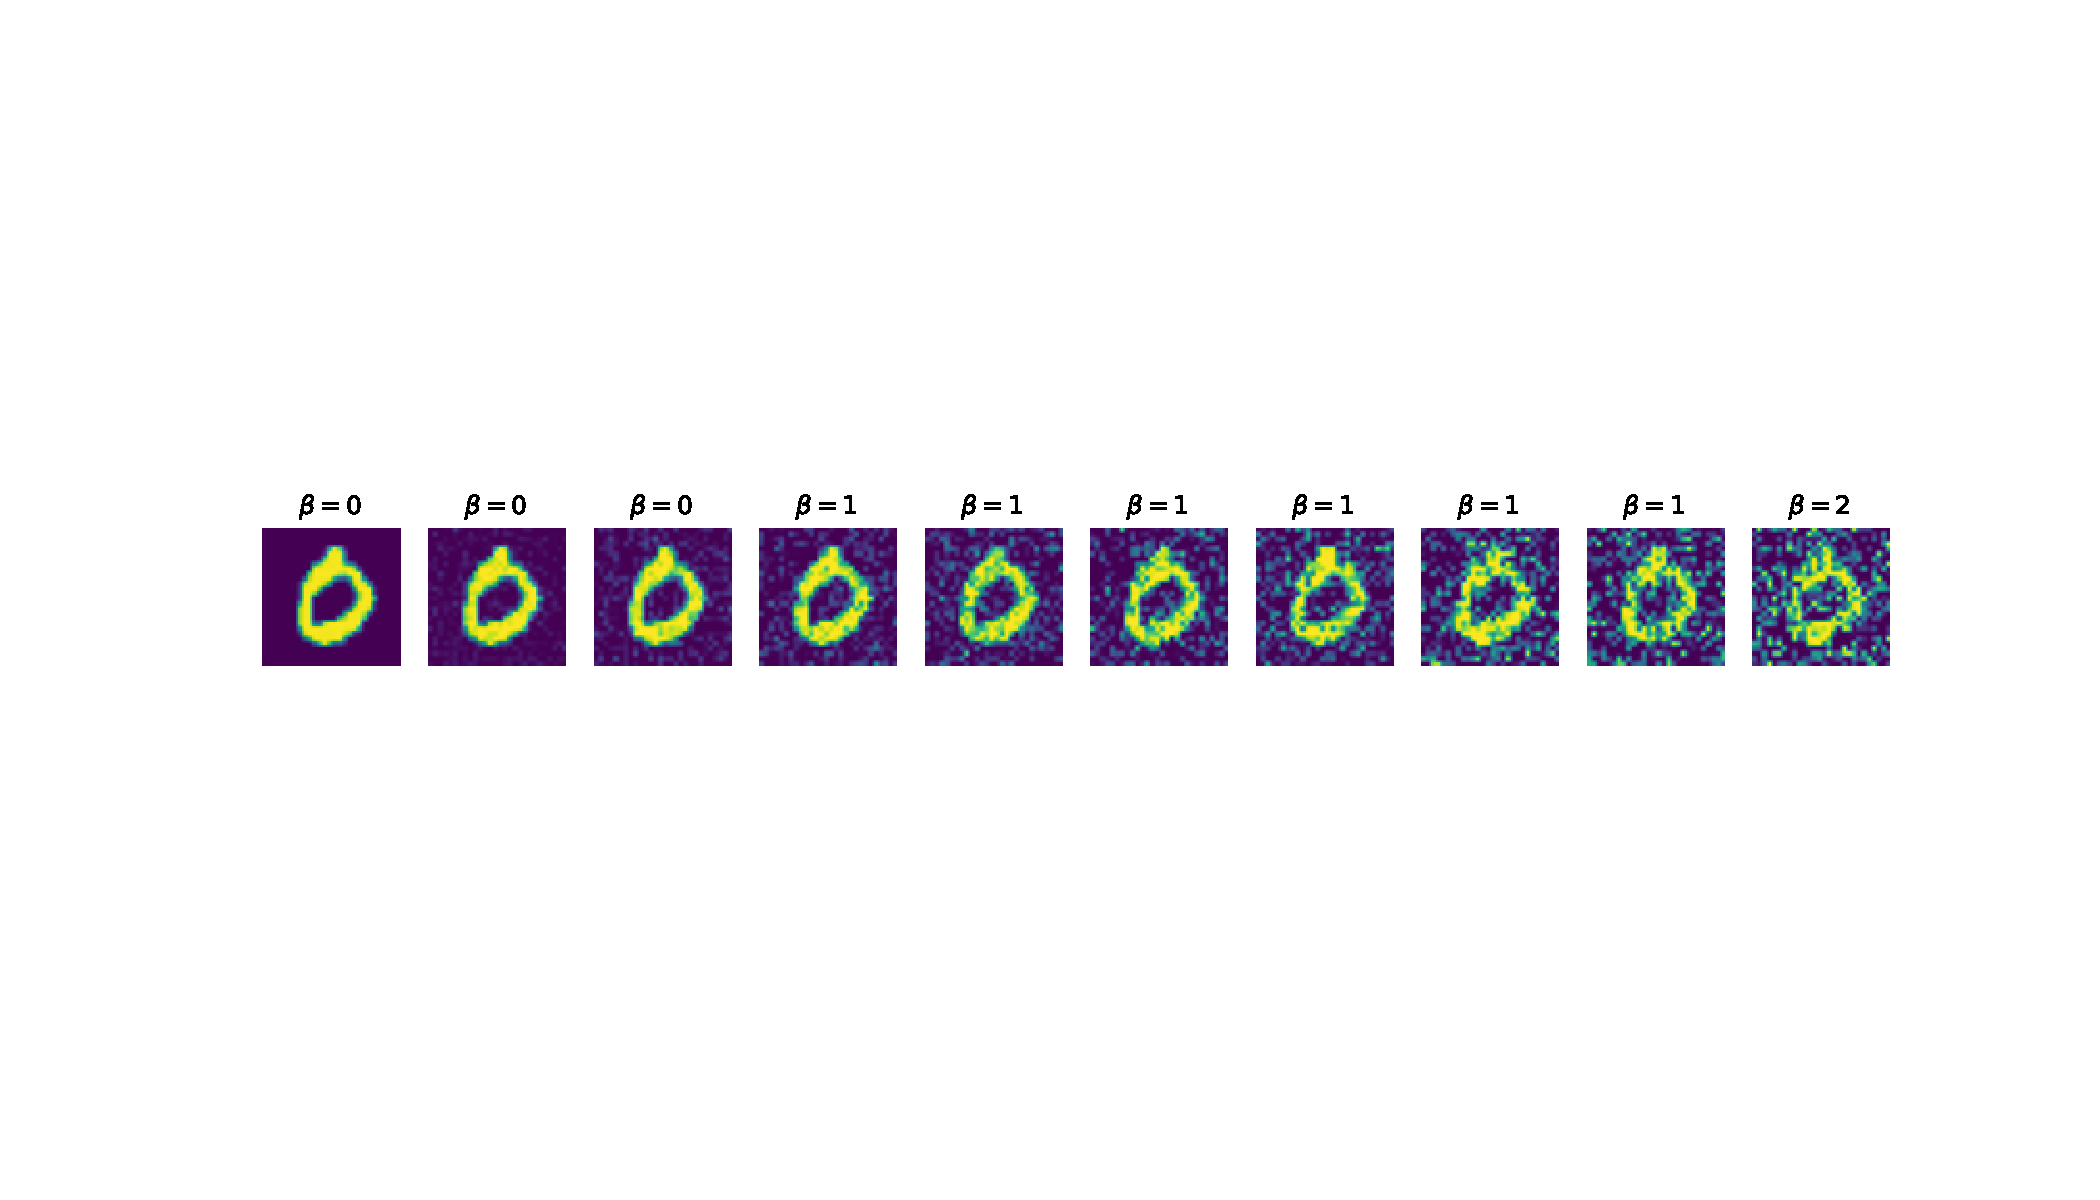
\includegraphics[trim=200 250 100 200, clip, width=\textwidth]{figures/samples_noise.pdf}
        \caption{Noise corruption of varying strength $\beta$.}
        \label{fig:samples_noise}
    \end{figure}
\end{frame}
\begin{frame}{Noise Corruption - Results}
    \doubleminipage{noise}{Accuracies of trained models under varying input noise corruption.}
\end{frame}

\begin{frame}{Blurring}
    $$
    \tilde {\vec x} = \text{gaussian\_blur} _\beta (\vec x)
    $$
    
    \begin{figure}[H]
        \centering
        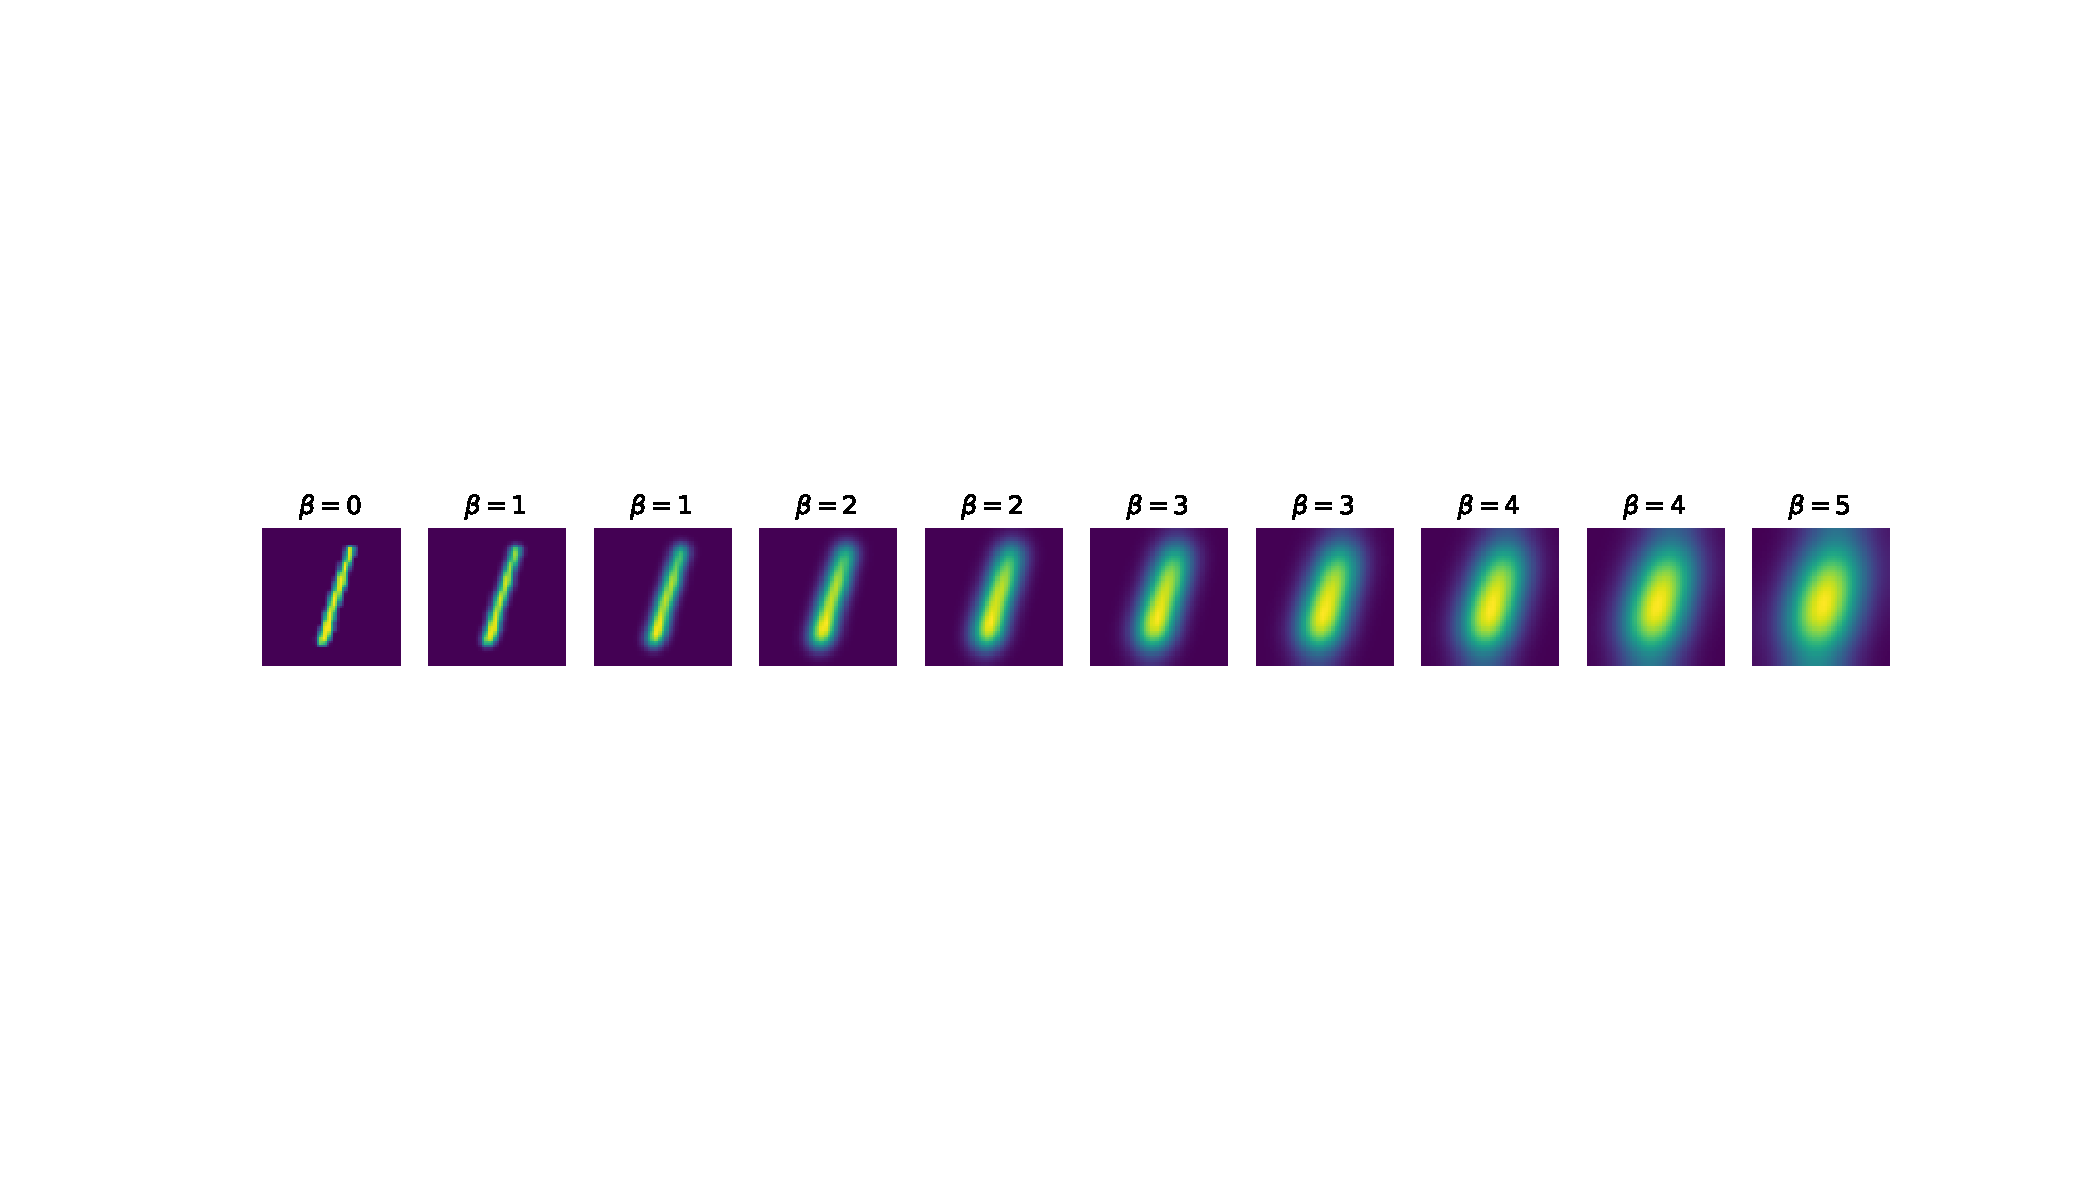
\includegraphics[trim=200 250 100 200, clip, width=\textwidth]{figures/samples_blur.pdf}
        \caption{Gaussian-blur filter applied with varying Gaussian kernel std $\beta$.}
        \label{fig:samples_blur}
    \end{figure}
\end{frame}
\begin{frame}{Blurring - Results}
    \doubleminipage{blur}{Accuracies of trained models under varying Gaussian-blur filters.}
\end{frame}

\begin{frame}{FGSM-Attack}
    \begin{align*}
    % \label{eq:fgsm}
    \begin{split}
    \vec x &\gets \vec x + \beta \, \text{sign}\left(\nabla_{\vec x} \mathcal L(D(\vec x), y)\right) \\
    \vec x &\gets \text{clip}[\, \vec x \,]
    \end{split}
    \end{align*}
    
    \begin{figure}[H]
        \centering
        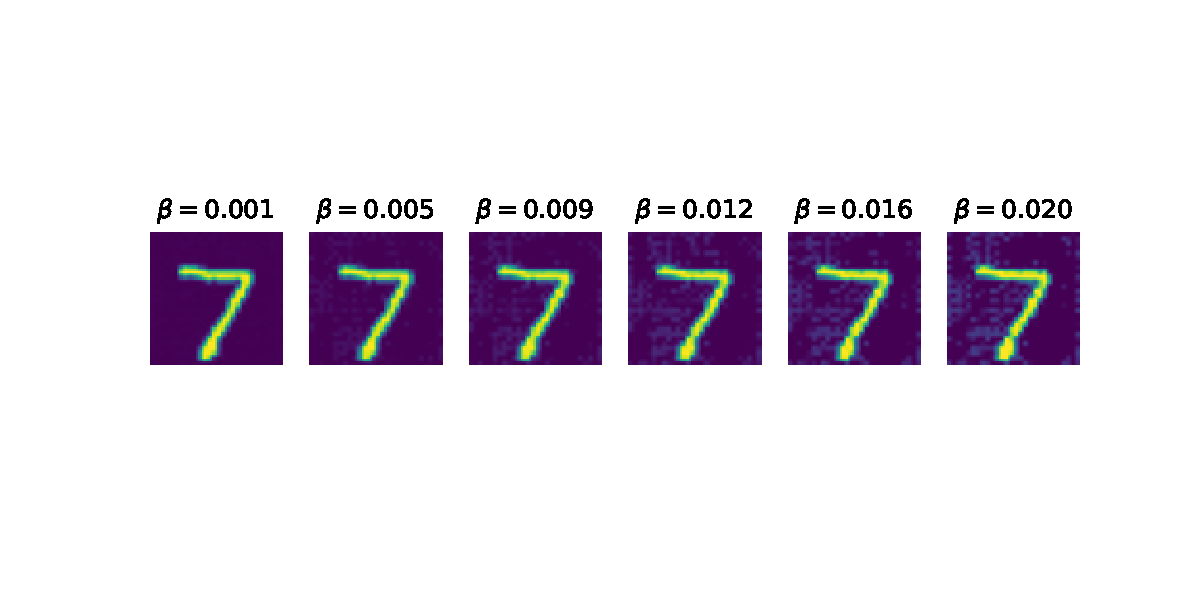
\includegraphics[trim=0 100 0 80, clip, width=0.8\textwidth]{figures/samples_fgsm.pdf}
        \caption{Results after 30 steps of FGSM-attack with varying $\beta$.}
        \label{fig:samples_fgsm}
    \end{figure}
\end{frame}
\begin{frame}{FGSM-Attack - Results}
    \doubleminipage{fgsm}{Accuracies of trained models under FGSM-attack with varying strengths.}
\end{frame}

\begin{frame}{LBFGS-Attack}
    \begin{align*}
    \label{eq:lbfgs}
    \begin{split}
    \vec x &\gets \vec x + \varepsilon \left( \nabla_{\vec x} \mathcal L(D(\vec x), y)
    - \frac 1 \beta \nabla_{\vec x} \| \vec x - \vec x^0 \|_2 \right) \\
    \vec x &\gets \text{clip}[\, \vec x \,]
    \end{split}
    \end{align*}
    
    \begin{figure}[H]
        \centering
        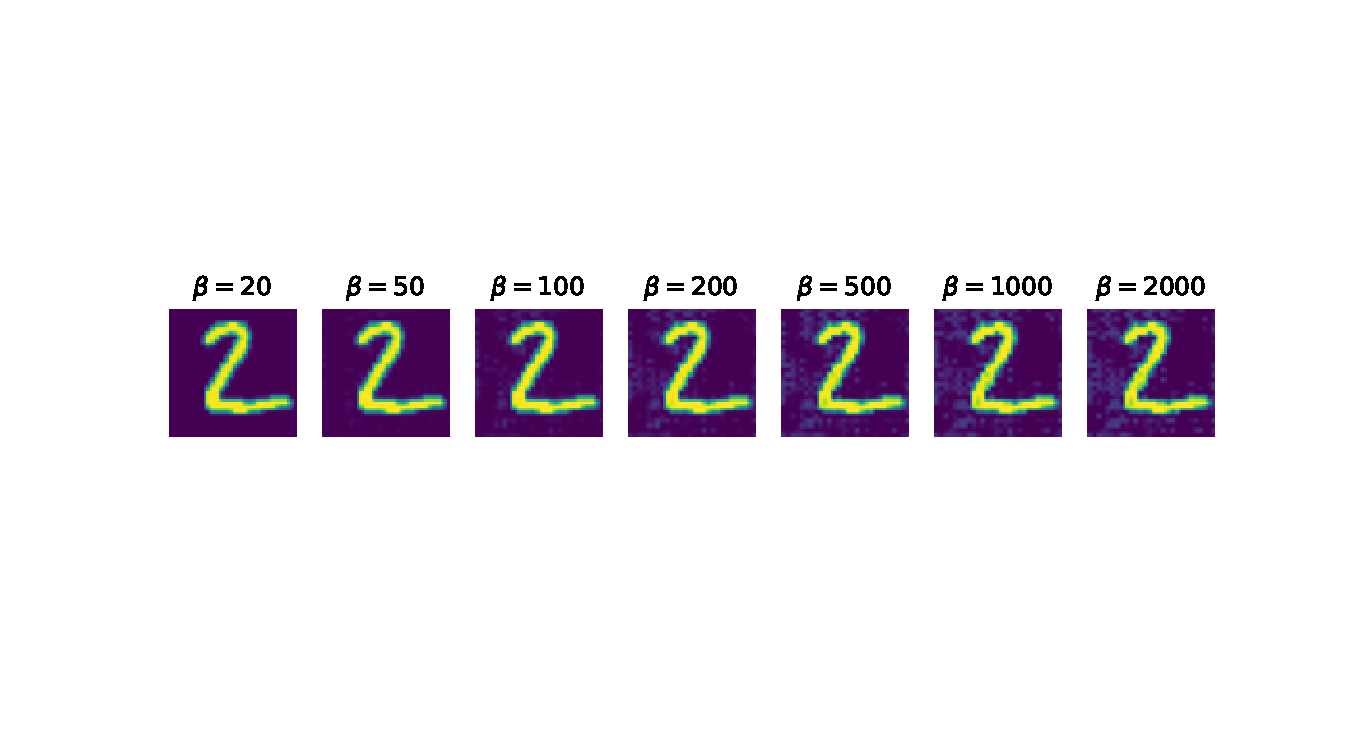
\includegraphics[trim=0 150 0 100, clip, width=\textwidth]{figures/samples_lbfgs.pdf}
        \caption{Results after 30 steps of LBFGS-attack with varying $\beta$.}
        \label{fig:samples_lbfgs}
    \end{figure}
\end{frame}
\begin{frame}{LBFGS-Attack - Results}
    \doubleminipage{lbfgs}{Accuracies of trained models under LBFGS-attack with varying strengths.}
\end{frame}

\section{Conclusion}

\begin{frame}{Conclusion}
    \begin{itemize}
        \item<1-> models trained with fewer GTN steps display
        (mostly) higher robustness
        \item<2-> models trained with GTNs are less robust than
        vanilla trained models
        \item<3-> however, number of testable architectures was limited due to shortcomings
        \item<4-> MNIST is a fairly simple task $\rightarrow$ more datasets are needed to be conclusive
        \item<5-> GTNs are likely to improve over time
    \end{itemize}
    
\end{frame}

{\setbeamercolor{palette primary}{fg=black, bg=Apricot}
\begin{frame}[standout]
  Questions?
\end{frame}
}

% \appendix


\begin{frame}[allowframebreaks]{References}
    \printbibliography
\end{frame}

\end{document}